\section{Brugergr�nseflade}

P� billederne \ref{write-message} og \ref{view-message} vises et udkast til applikationens brugergr�nseflade.

Vinduet p� billede \ref{write-message} benyttes af bes�gende til at skrive beskeder til en g�stebog. Sammen med beskeden indtastes et navn, og brugeren har mulighed for at bed�mme sit ophold.

Vinduet p� billede \ref{view-message} kan bruges af andre bes�gende eller administratoren til at se de beskeder, som tidligere er blevet tilf�jet til en g�stebog.

\begin{figure}
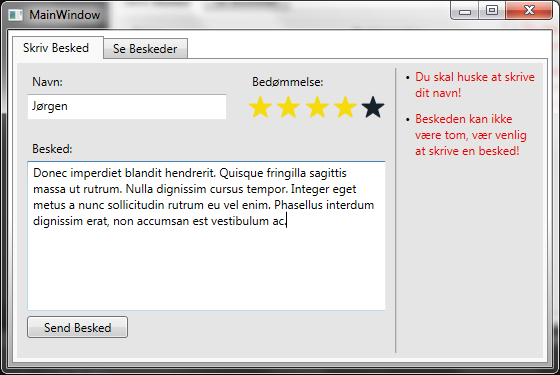
\includegraphics[width=\linewidth]{../Skriv_Besked}
\caption{Vinduet til at skrive en besked}
\label{write-message}
\end{figure}

\begin{figure}
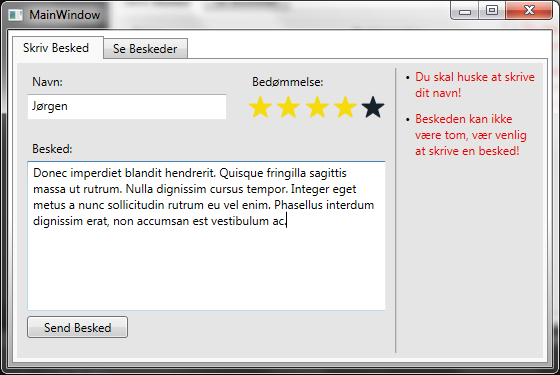
\includegraphics[width=\linewidth]{../Se_Beskeder}
\caption{Vinduet hvor alle beskeder kan ses}
\label{view-message}
\end{figure}